
Il mio compito nello sviluppo dell'applicazione è stato quello 
di creare un \textbf{prototipo} iniziale avendo a disposizione un mock up creato con
proto.io\cite{protoio} e una serie di requisiti essenziali.

\subsection{Mock up iniziale}

Il prototipo iniziale dell'applicazione prevede una
bottom TabBar con cinque elementi ognuno dei quali
descrivere le seguenti funzionalità:

\begin{enumerate}
    \item \textbf{Storico delle offerte}: è stato implementato attraverso un pattern Overview and Details
    e consiste in una lista in cui l'utente può visualizzare i dettagli cliccando sull'offerta desiderata.
    \item \textbf{Tutte le offerte}: la vista è strutturata con un filtro per categoria nella parte superiore,
    con cui l'utente può controllare tutte le offerte disponibili. Tutte le offerte offrono una tipologia di QIX Shake diversa tra quelle elencate nell'introduzione.
    \item \textbf{Sezione Scan}: la sezione scan sarà utilizzata per lo scanning di QR Code o di scontrini d'acquisto da parte dell'utente,
    così che possa guadagnare dei QIX Coins.
    \item \textbf{Gift Cards}: in questa sezione l'utente potrà comprare delle gift cards digitali o materiali usando i suoi QIX Coins.
    \item \textbf{Sezione Me}: in questa view vengono mostrati tutti i dati riguardanti l'utente, il supporto tecnico
    e la funzione per invitare gli amici.
\end{enumerate}

Oltre alle viste principali ho creato anche un onboarding in cui l'utente può decidere se effetture la registrazione
attraverso il proprio numero di telefono o entrare direttamente nell'app come utente Guest, un esempio della registrazione è
visibile nell figura~\ref{fig:screenshots} (d).

\begin{figure}
    \hfill
    \subfigure[Storico offerte]{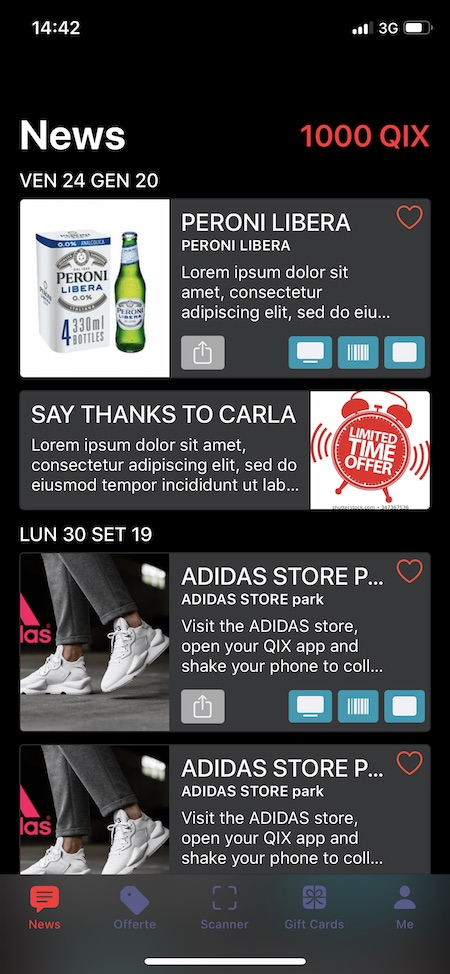
\includegraphics[width=3.2cm]{screen_1}}
    \hfill
    \subfigure[Tutte le offerte]{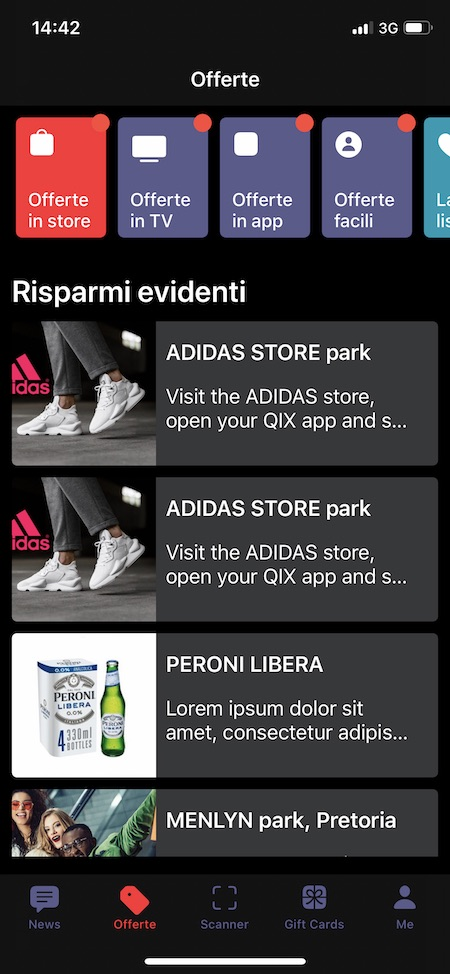
\includegraphics[width=3.2cm]{screen_2}}
    \hfill
    \subfigure[Sezione Me]{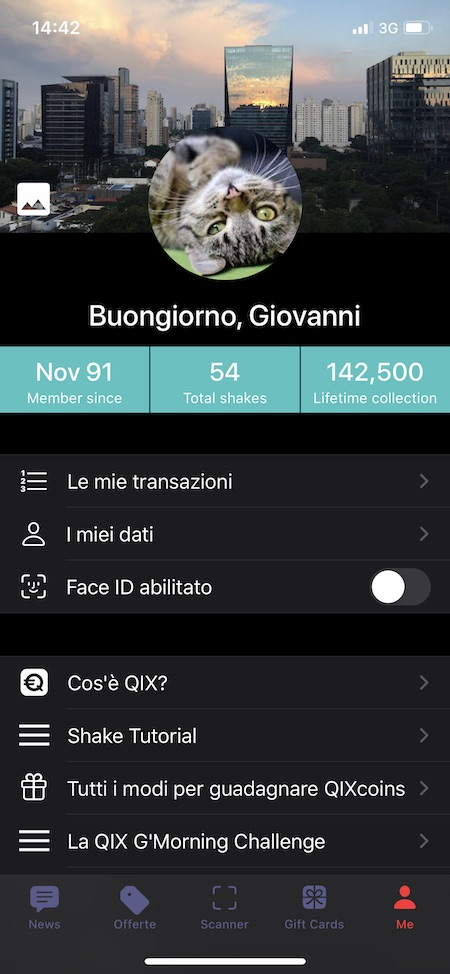
\includegraphics[width=3.2cm]{screen_3}}
    \hfill
    \subfigure[Registrazione]{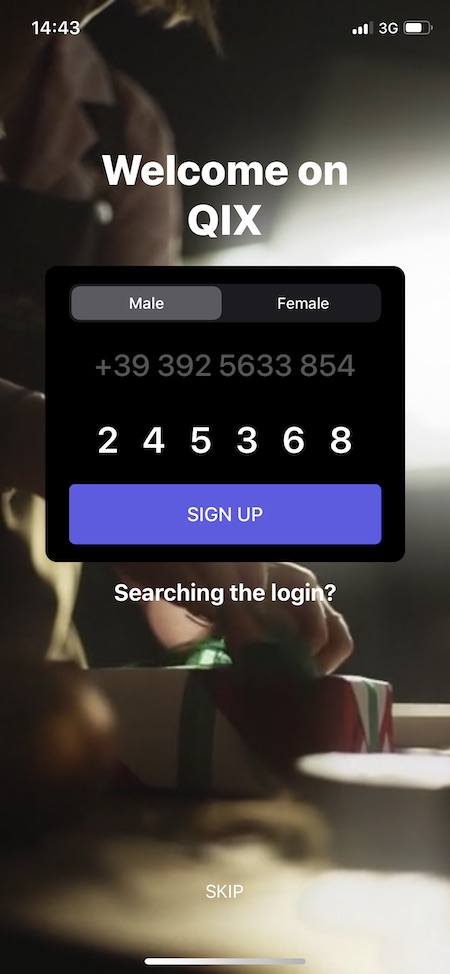
\includegraphics[width=3.2cm]{screen_4}}
    \hfill
    \caption{Screenshots prototipo iniziale}\label{fig:screenshots}
\end{figure}

In particolare, come spiegherò nella sezione~\ref{sec:coordinator}, è stato utilizzato il Coordinator Pattern
per la gestione delle viste ed ogni view visibile in figura~\ref{fig:screenshots} è un esempio di UIViewController
figlio di un CoordinatorNavigable.

\subsection{Requisiti}
La base di partenza di QIX sono state delle funzionalità essenziali e 
sostanzialmente molto difficili da inserire in una versione dell'app già avanzata.
È stato quindi deciso di creare un prototipo di partenza avente i seguenti requisiti:

\begin{itemize}
    \item {
        \textbf{Navigazione dinamica}: L'applicazione deve gestire dei cambiamenti di contesto
        dinamici: dev'essere possibile mostrare all'utente contenuti dinamici indipendentemente
        dal contesto in cui si trova. 
    }
    \item {
        \textbf{QIX Shake}: L'utente deve poter agitare lo smartphone in qualsiasi
        sezione dell'applicazione e il risultato deve essere basato sul contesto attuale o su delle direttive dettate
        da delle Rest API.
    } 
    \item {
        \textbf{Animazioni interattive}: L'intera applicazione dev'essere progettata in modo tale da presentare all'utente
        delle \textbf{animazioni interattive} in stile CardView\cite{cardview} disponibili in 
        qualunque sezione o vista in cui si trovi l'utente e definite dal contesto attuale.

        Le animazioni in questione devono essere progettate in pagine, ciascuna delle quali può contenere 
        più CardView. L'utente vedrà in un determinato momento una e soltanto una pagina.

        Ogni CardView deve essere trascinabile dall'utente e deve interagire con le altre CardView della pagine. 
        Quando l'utente usa una forza di trascinamento superiore a un valore di soglia tutte le viste devono
        cadere per gravità.
        
        Tale gravità finirà con la fine dell'animazione o l'apparizione di una nuova pagina se presente.
    }
    \item {
        \textbf{Autenticazione}: L'applicazione deve supportare tre diversi stati o modalità di autenticazione:
        \begin{enumerate}
            \item\textbf{Trial Mode}: l'utente è anonimo, esiste solo un id per tenere traccia dei suoi QIX coins.
            \item\textbf{Signed Mode}: l'utente ha inserito il numero di telefono e il suo genitore.
            \item \textbf{Pro Mode}: l'utente aggiunge dei dati su se stesso o collega il suo account a dei social media come Facebook, Google o Instagram.
        \end{enumerate}
        Si nota facilmente che non esiste una stato in cui l'utente non è registrato: questo perchè
        per tenere traccia dei suoi QIX coins e di altri dati utili è necessario avere una riferimento all'utente.
    }
    \item {
        \textbf{DeepLinks}: L'applicazione deve poter essere avviata dinamicamente
        attraverso dei \textbf{Deep Links}\cite{deeplinks}.
        E deve essere in grado di gestirli in base al contesto dell'utente.
    }
\end{itemize}